%
% File acl2019.tex
%
%% Based on the style files for ACL 2018, NAACL 2018/19, which were
%% Based on the style files for ACL-2015, with some improvements
%%  taken from the NAACL-2016 style
%% Based on the style files for ACL-2014, which were, in turn,
%% based on ACL-2013, ACL-2012, ACL-2011, ACL-2010, ACL-IJCNLP-2009,
%% EACL-2009, IJCNLP-2008...
%% Based on the style files for EACL 2006 by 
%%e.agirre@ehu.es or Sergi.Balari@uab.es
%% and that of ACL 08 by Joakim Nivre and Noah Smith

\documentclass[11pt,a4paper]{article}
\usepackage[hyperref]{acl2019}
\usepackage{times}
\usepackage{latexsym}
\usepackage{amsmath}
\usepackage{multirow}
\usepackage{pgfplots}
\usepackage{pgfplotstable}
\pgfplotsset{compat=1.7}
\usepackage{tikz}
\usepackage{lipsum}% http://ctan.org/pkg/lipsum
\usepackage{graphicx}% http://ctan.org/pkg/graphicx

\usepackage{url}

\aclfinalcopy % Uncomment this line for the final submission
%\def\aclpaperid{***} %  Enter the acl Paper ID here

%\setlength\titlebox{5cm}
% You can expand the titlebox if you need extra space
% to show all the authors. Please do not make the titlebox
% smaller than 5cm (the original size); we will check this
% in the camera-ready version and ask you to change it back.

\newcommand\BibTeX{B\textsc{ib}\TeX}
\title{Fluorescing\thanks{  Cosine Similarity of Fluoresce and Answer: $0.89$} Questions: Effects of Semantic Perturbations on BERT Performance in SQuAD 1.1}

\author{\normalfont \textbf{Spencer Ng}, \textbf{Lucy Teaford}, \textbf{Andy Yang}, and \textbf{Isaiah Zwick-Schachter} \\
 \texttt{\{spencerng,lteaford,andyjyang,isaiahzs\}@uchicago.edu} \\
 CMSC 25610: Computational Linguistics \\
 University of Chicago}

\date{December 10, 2021}

\begin{document}
\maketitle

% \begin{abstract}
%   This document contains the instructions for preparing a camera-ready
%   manuscript for the proceedings of ACL 2019. The document itself
%   conforms to its own specifications, and is therefore an example of
%   what your manuscript should look like. These instructions should be
%   used for both papers submitted for review and for final versions of
%   accepted papers.  Authors are asked to conform to all the directions
%   reported in this document.
% \end{abstract}



\section{Introduction}

It has long been an outstanding question whether language models have an internal ``understanding'' of human language or if they are performing some kind of clever pattern matching to make linguistic predictions. In particular, we focus on the degree to which language models rely on the semantic meaning of verbs. For example, if we query a language model for the answer to the question ``What year was Beyoncé born in?'', will it produce the result ``1981'' because it found ``1981'' in conjuction with the verb ``born,'' or simply because ``1981'' is a year and it made a guess? In particular, if we query the question ``What year was Beyoncé photocopied in?'', how will that affect the language model prediction?

We propose to evaluate a question answering model with adversarially generated semantic perturbations on verbs in the test sets, in order to see the degree to which the model's success relies on the semantic meanings of verbs which it encounters. The intensity of semantic perturbation will be incremented in a controlled manner, in order to evaluate the degree to which model behavior is dependent on the semantic meaning of verbs. 

More specifically, in this paper we consider whether Bidirectional Encoder Representations from Transformers (BERT), a language representation model from researchers at Google AI Language, relies significantly on verb semantics in order to answer questions in the Stanford Question Answering Dataset (SQuAD 1.1). Taking inspiration from \citet{gulordava-etal-2018-colorless} and \citet{jia2017adversarial}, we evaluate BERT using adversarially generated test examples of SQuAD 1.1 to determine the properties of its prediction procedure. We train BERT on SQuAD 1.1 to establish a baseline for its performance in answering questions. Then, we generate a set of semantically perturbed but syntactically unchanged test examples by swapping in verbs at differing levels of cosine similarity to the original. This is achieved using a pre-trained word vector model. We evaluate BERT’s performance in answering these new semantically perturbed questions to determine whether verb meaning contributes to BERT’s understanding of the task. We hypothesize that BERT’s performance would change significantly, decreasing in performance as verbs in questions are replaced with increasingly dissimilar verbs, indicating that BERT relies on semantics beyond sentence structure to answer questions.

% An Introduction that sets up the problem you're addressing, why it matters (often contextualized briefly with respect to relevant literature), how you plan to approach it, and a brief summary of what you found.

\section{Related Work} \label{related work}

Our project is jointly inspired by \citet{gulordava-etal-2018-colorless} and \citet*{jia2017adversarial}.

\subsection{Gulordava et al.} 
 Like Gulordava et al., we are interested in evaluating what a language model learns about language during training. By testing a recurrent long short term memory (LSTM) language model on sensitivity to subject-verb and long-distance number agreement in semantically nonsensical sentences, Gulordava et al. were able to conclude that training on a language acquisition objective is enough to trigger syntactic learning in a recurrent LSTM language model without built-in linguistic knowledge. In our project, we tested for semantic learning in a bidirectional transformer model.

\subsection{Jia and Liang} 
While Gulordava et al. replaced each content word with a random, morphologically equivalent content word to create nonce versions of each original input sentence, we were inspired by Jia and Liang to narrow our focus to explicitly adversarial verbs. Jia and Liang, who also evaluate model performance on SQuAD, emphasize the importance of a precise adversarial evaluation scheme in determining what a model truly understands about language.

\subsection{Syntax and Semantics: Are they distinct?}

We recognize that syntax and semantics are, to an extent, interdependent, and it is difficult to cleanly separate the syntactic and semantic representations of a question. \citet{de_bot_lowie_verspoor_2007} assert that language is a dynamic system with complete interconnectedness between its subsystems, which include syntax and semantics. Also calling on dynamic systems theory, \citet{ART002728950} claims that the syntactic-semantic space is the only level of representation in language, and that syntactic and semantic language processing cannot be distinguished. \citet{DBLP:journals/corr/abs-1711-02013} propose a novel neural language model, Parsing-Reading-Predict Networks (PRPN), that learns the syntactic structure of sentences, then uses this structural information to form better semantic, or word meaning, representations. The proposed mechanism underlying this model suggests an interconnectedness between syntax and semantics.

However, we are encouraged by literature that suggests a distinction between syntax and semantics. \citet{ek-etal-2019-language} trained LSTM language models on sentences annotated with syntactic roles and semantic information, and they found that only the syntactic tags lowered the perplexity of the models. \citet{DBLP:journals/corr/abs-2104-05115} present ParaBART, a sentence embedding model that learns to disentangle syntax and semantics in input  sentences through paraphrasing. \citet{mitchell-steedman-2015-orthogonality} found that distributional models produce word representations that are decomposed into orthogonal syntactic and semantic spaces. 

Given these findings, we are confident that language representation models are capable of differentiating syntactic and semantic information during training, and that these subsets of information have distinguishable effects on the success of these models in completing natural language understanding tasks.

% Optionally you can include a description of Related Work and how your project is situated with respect to existing literature. In a standard paper this section would be critical, but for the purpose of this project I am making literature review optional.

\section{Methods}

\subsection{Task}

The SQuAD 1.1 dataset is designed to evaluate reading comprehension, consisting of a series of ``context'' paragraphs drawn from 536 English Wikipedia articles and a series of questions whose answers can be found as a segment of text from the corresponding article \cite{rajpurkar2016squad}. Questions and their related paragraph are provided as inputs to natural language processing models, which then extract the answer from the provided paragraph. We use the publically-available SQuAD 1.1 dataset for our experiments, training on 19,047 paragraphs of context and their associated 87,599 questions from the training set. For evaluating our model and creating perturbed questions and contexts, we used the dev set, consisting of 10,570 questions and 2,137 related paragraphs.

\subsection{Model}

We trained and evaluated a baseline model finetuned from a pretrained BERT uncased language model and tokenizer using the Huggingface Transformers library \cite{wolf-etal-2020-transformers}. The bidirectional BERT model is used because it is well-suited to accurately model downstream tasks, and the parameter fine-tuning process is relatively inexpensive \cite{devlin2019bert}. The BERT model was trained for three epochs on the SQuAD 1.1 training set, using a learning rate of $2\cdot 10^{-5}$, a batch size of 4, and a weight decay of 0.01. Our baseline model achieves an accuracy of 80.04\%.

Example contexts and questions were broken into tokens (text spans) of at most 384 characters, and the start and end indices of ground truth answers within paragraph contexts were fed into the model. For generating predictions and evaluation, a similar process was followed, where tokens were generated from questions and contexts, and the model output a vector of probabilities $S$ and $E$ corresponding with each character in the tokenized context. Each probability $S_i$ and $E_j$ then corresponded with the chance of the $i$th character in the context span being the first character of the answer to the question and the $j$th character being the last character of the answer. We apply a softmax function to each vector to find the most likely start and end locations for the answer, ensuring that $i< j$, and outputting the character sequence with the $i$th through $j$th characters from the span as the answer. If no valid prediction is found, we output an empty string as the answer.

\subsection{Semantic Perturbation}
To control for a model's sensitivity to syntactic structure while testing its sensitivity to semantic perturbation, we used the following procedure to modify the meaning of a piece of text while preserving its syntactic structure:
\begin{enumerate}
    \item Select a verb $v$ from a piece of text
    \item Lemmatize $v$. 
    \item Use a word-vector model to find a second verb $v'$ at a desired cosine similarity distance from the lemmatized $v$
    \item replace $v$ in the text with $v'$
\end{enumerate}

In this way, we can ensure that the syntax of the text remains constant while the semantic meaning changes. We use the NLTK library \cite{bird2009natural} for tokenizing sentences, tagging words with their POS, and lemmatizing verbs. Verb tenses that the NLTK tagging library could recognize included were past tense, present participle, past participle, non-3rd person singular present, and 3rd person singular present. 

We use the gensim library \cite{rehurek2011gensim} for computing verbs of desired cosine similarity values. We imported the WebVectors enwiki\_upos\_skipgram\_300\_3\_2019 model
\cite{kutuzov2017word} to use as our word vector model. This is a Gensim Continuous Skipgram model, trained on the English Wikipedia dump of October 2019. It contains $249212$ different words, tagged by part of speech. The choice of a vector model trained on Wikipedia articles is to keep our verb transformations within the same register, as SQuAD1.1 is also from Wikipedia,  Given a verb $v$, we find other verbs $v'$ of varying cosine similarities to $v$ by iterating through the verbs in the model. 

To conjugate verbs into the desired tense we use the mlconjug library \cite{mlconjug3}. This allows us to take a verb $v'$ of the desired cosine similarity to our original verb, give it the same syntactic category as the verb it is to be replacing, and then insert it into the text. 

Through manual inspection we verified that this process was successful at creating sentences that were semantically different but syntactically similar to the original. In particular, as the cosine similarity of the transformed verb decreases, the inspected semantic meaning becomes more and more anomalous. An example of this is placed in Table 1. 

\begin{table}
\centering
\small

\begin{tabular}{|p{2.35cm}|p{4.4cm}|}
\hline
\textbf{Cosine Similarity} & \textbf{Question}\\\hline
\verb$1.0$ & \texttt{What percentage of Australia's dairy cattle are \textbf{found} in Victoria?}\\\hline
\verb$0.6$ & \texttt{What percentage of Australia's dairy cattle are \textbf{identified} in Victoria?}\\\hline
\verb$0.5$ & \texttt{What percentage of Australia's dairy cattle are \textbf{searched} in Victoria?}\\\hline
\verb$0.4$& \texttt{What percentage of Australia's dairy cattle are \textbf{disproved} in Victoria?}\\\hline
\verb$0.3$ & \texttt{What percentage of Australia's dairy cattle are \textbf{uncoound} in Victoria?}\\\hline
\verb$0.2$ & \texttt{What percentage of Australia's dairy cattle are \textbf{fluoresce/outbidden} in Victoria?}\\\hline
\end{tabular}

\caption{Question id $=3006$ modified at varying levels of verb cosine similarity ($1.0$ indicates the original question in the SQuAD1.1 test set).}\label{tab:accents}
\end{table}


\subsection{Data Preparation}

To prepare the data for our experiments, we needed to process it into a format that was more easily consumable by our models and our verb substitution process. To do this, we first extracted the training set to feed it to our models, and then we extracted and processed the test (dev) set to use to evaluate out models. We extracted question answer pairs for easier verb substitution and we processed each question answer grouping into a category. All questions in the SQuAD 1.1 dataset belong to one of 10 categories: ``date,'' ``other numeric,'' ``person,'' ``location,'' ``other entity,'' ``common noun phrase,'' ``adjective phrase,'' ``verb phrase,'' ``clause,'' or ``other.'' 

We could not locate a dataset that tagged the questions for us, so we categorized them ourselves. We did this by examining questions in the test/dev dataset by hand and guessing at patterns that could be easily checked to determine a questions category. There were several patterns that appeared to be reliable indicators of the questions category, for example questions containing ``how many'' will typically have ``numeric'' answers and questions asking about a date/year/month will typically be referring to a date. Based on our manual examination of questions and extending that using regular expression patterns, we classified approximately 1800 questions, accounting for nearly 20\% of the questions  in the test/dev set. Getting a measure of our accuracy would be challenging, since these were already hand classified, but we estimate about 75\% accuracy on the questions we could determine a category for. The other ~8000 that we could not classify were categorized as ``other''.

\subsection{Evaluation}

To evaluate the accuracy of our model on both the baseline test set and perturbed examples, we compute accuracy and F1 score metrics.

Given our fine-tuned model $f$ and a set of test questions $Q$, related contexts $C$, and ground truth answers $\mathcal{A}$, we define $\hat{A}$ to be the set of answers predicted by $f$, where $\hat{a}_i=f(q_i, c_i)$ is the predicted answer to the $i$th question in $Q$, which has an associated context $c_i$. We then apply a normalizing function $n$ to each $\hat{a}_i\in \hat{A}$, where we remove articles, punctuation, and white space from answers. We also ensure each predicted answer and associated set of ground truth answers $A_i \in \mathcal{A}$ is converted to lowercase to account for the original uncased BERT model. This normalizing function $n$ is borrowed from the official evaluation script from \citet{rajpurkar2016squad}.

The \textit{accuracy} as reported in our results for a given test set $T=(Q, C, A)$  is then equal to
\begin{align*}
    \text{acc}(T) = \frac{1}{|Q|} \sum_{q_i \in Q} \begin{cases}
        1 & \text{if } f(q_i, c_i) \in A_i \\
        0 & \text{otherwise} \\
    \end{cases}
\end{align*}

Similarly, the F1 score is equal to
\begin{align*}
    \text{F}_1(T) = \frac{1}{|Q|} \sum_{q_i \in Q} \text{F}_{1_a}(f(q_i, c_i), A_i),
\end{align*}
where $\text{F}_{1_a}$ is the F1 function provided by \citet{rajpurkar2016squad} that measures the m.aximum overlap between a given prediction predicted answer $\hat{a}_i$ and all ground truth answers $a \in A_i$.

To compute the accuracy and F1 score for a given category of questions in our analysis, we take a subset of the test set questions and associated contexts $Q' \subset Q$ that belong in that category.

\section{Experiments}

After training BERT on the SQuAD 1.1 question and answer task, we generate adversarial examples to evaluate the model upon. The original SQuAD 1.1 test set contains $10570$ questions, each referring to one of $2067$ paragraphs. Three classes of test sets were generated from the original: one modifying only the questions, one modifying only the paragraphs, and one modifying both. Within each class, we generated $5$ different gradations of semantic perturbation. We run BERT on these test sets in order to evaluate the effect of different kinds and degrees of verb perturbation. 

\begin{figure*}[h]
\centering
\begin{tabular}{ |m{1.75cm}|c|c|c|c|c|c|c|c|c|c|c|c| }
  \hline
  \textbf{Cos. Similarity} & \multicolumn{2}{|c|}{\textbf{Baseline}} &
  \multicolumn{2}{|c|}{\textbf{0.2}} &
  \multicolumn{2}{|c|}{\textbf{0.3}} &
  \multicolumn{2}{|c|}{\textbf{0.4}} &
  \multicolumn{2}{|c|}{\textbf{0.5}} &
  \multicolumn{2}{|c|}{\textbf{0.6}}\\
  \cline{1-13}
  Result & F1 & acc & F1 & acc & F1 & acc & F1 & acc & F1 & acc & F1 & acc \\
  \hline
  Question Only & 87.79 & 80.04 & 83.48 & 75.01 & 81.81 & 73.46 & 82.51 & 74.20 & 85.76 & 77.73 & 86.14 & 78.25\\
  \hline
  Context Only & 87.79 & 80.04 & 84.36 & 74.27 & 85.40 & 76.36 & 85.66 & 76.92 & 86.27 & 77.69 & 86.61 & 78.16\\ 
  \hline
  Question + Context & 87.79 & 80.04 & 81.81 & 72.04 & 80.96 & 71.94 & 81.98 & 72.92 & 85.18 & 76.59 & 85.88 & 77.44\\
  \hline
\end{tabular}
\caption{F1 and accuracy results for increasing levels of cosine similarity when only the question is modified, only the context is modified, or both the question and context are modified.}
\label{tab:my_label}
\end{figure*}

\subsection{Generating Semantically Perturbed Examples}



 The generated semantic perturbations followed the process outlined in the methods section in the manner described below:

 \textbf{Questions:} The last verb in each given question was perturbed.
 
 \textbf{Paragraphs:} For every question which refers to a given paragraph, we find occurrences of the last verb in the question within the paragraph. Each of these occurrences is replaced with the verb which replaces the question's verb. We insure that each replacement verb in the paragraph is in the same tense as the original verb.

\begin{table}[h]
\centering
\small

\begin{tabular}{|p{3.5cm}|p{3.5cm}|}
\hline
\textbf{Original} & \textbf{Perturbed}\\\hline
\texttt{Warsaw \textbf{is} located on two main geomorphologic formations \ldots which \textbf{divides} the city into two parts, left and right. The left one  \textbf{is}  situated both on the moraine plateau \ldots \textbf{called} Warsaw Escarpment. It  \textbf{is}  20 to 25 m (65.6 to 82.0 ft) high in the Old Town \ldots} & \texttt{Warsaw \textbf{needs} located on two main geomorphologic formations \ldots which \textbf{edomiinds} the city into two parts, left and right. The left one  \textbf{needs} situated both on the moraine plateau \ldots \textbf{tound} Warsaw Escarpment. It  \textbf{needs} 20 to 25 m (65.6 to 82.0 ft) high in the Old Town\ldots}\\\hline
\end{tabular}

\caption{Excerpt of paragraph id $=87$ modified with a verb cosine similarity of $0.4$, replacing the the verbs which occur in the questions referring to said paragraph.}\label{tab:accents}
\end{table}

In this manner, the modified questions and modified paragraphs are intended to be consistent with each other. 

Within the English Wikipedia 2019 word vector model, the cosine similarity between any given verbs generally ranges between $0.2$ and $0.6$. For this reason, we generated $5$ different semantically perturbed test sets, substituting in verbs at the following different levels of cosine simililarity: $0.6,0.5,0.4,0.3,0.2$. Table 1 illustrates a semantically perturbed question, Table 2 illustrates an example of a semantically perturbed paragraph.





\section{Results}



\begin{figure}[h]
\centering
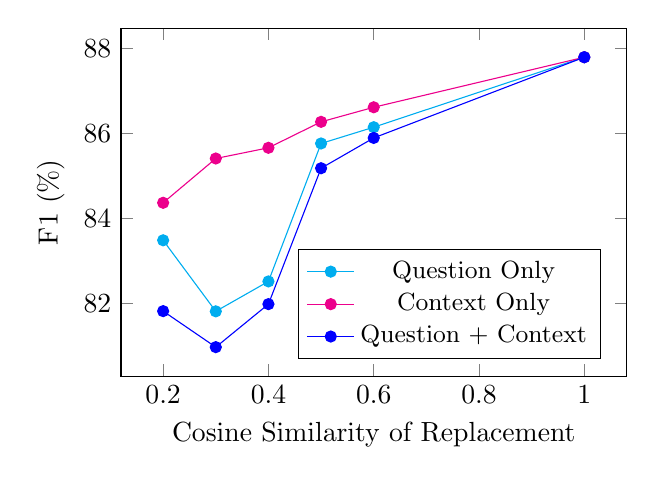
\begin{tikzpicture}
\begin{axis}[
	xlabel=Cosine Similarity of Replacement,
	ylabel=F1 (\%),
	width=8cm,height=6cm,
    legend style={at={(0.95,0.05)},anchor=south east,font=\small}
    ]

% Add values and attributes for the first plot
\addplot[color=cyan,mark=*] coordinates {
	(0.2, 83.4791390201524)
	(0.3, 81.8060595606836)
	(0.4, 82.5107370623591)
	(0.5, 85.7588204117612)
	(0.6, 86.1414660497779)
	(1.0, 87.7893481205936)
};

% Add values and attributes for the second plot
\addplot[color=magenta,mark=*] coordinates {
    (0.2, 84.3620769918265)
	(0.3, 85.4047552706945)
	(0.4, 85.6565606212204)
	(0.5, 86.2677545259184)
	(0.6, 86.6108625069709)
	(1.0, 87.7893481205936)
};

\addplot[color=blue,mark=*] coordinates {
    (0.2, 81.8111826043422)
	(0.3, 80.9632864951269)
	(0.4, 81.976105201615)
	(0.5, 85.1758289720334)
	(0.6, 85.8890240572509)
	(1.0, 87.7893481205936)
};

\legend{Question Only, Context Only, Question + Context}
\end{axis}
\end{tikzpicture}
\caption{F1 (\%) for increasing levels of cosine similarity when only the question is modified, only the context is modified, or both the question and context are modified.}
\end{figure}



\begin{figure}[h]
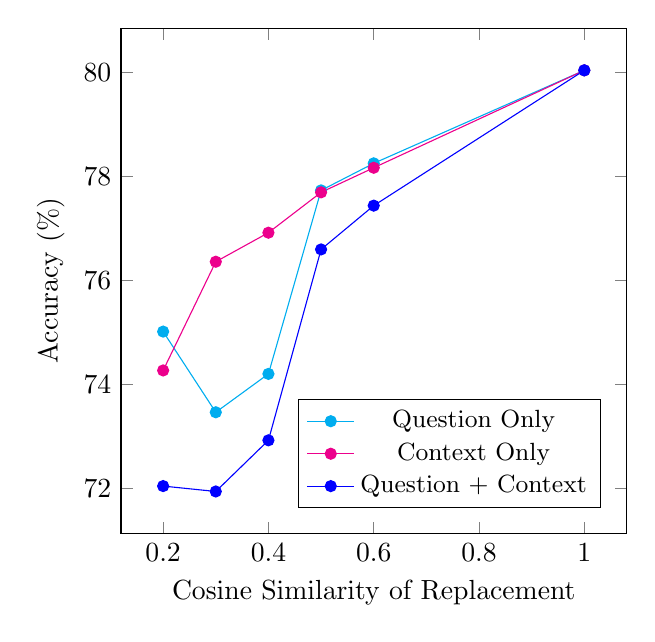
\begin{tikzpicture}
\begin{axis}[
	xlabel=Cosine Similarity of Replacement,
	ylabel=Accuracy (\%),
	width=8cm,height=8cm,
    legend style={at={(0.95,0.05)},anchor=south east,font=\small}
    ]

% Add values and attributes for the first plot
\addplot[color=cyan,mark=*] coordinates {
	(0.2, 75.0141911069063)
	(0.3, 73.4626300851466)
	(0.4, 74.2005676442763)
	(0.5, 77.7294228949858)
	(0.6, 78.2497634815516)
	(1.0, 80.0378429517502)
};

% Add values and attributes for the second plot
\addplot[color=magenta,mark=*] coordinates {
    (0.2, 74.2667928098392)
	(0.3, 76.3576158940397)
	(0.4, 76.9157994323557)
	(0.5, 77.6915799432356)
	(0.6, 78.1646168401135)
	(1.0, 80.0378429517502)
};

\addplot[color=blue,mark=*] coordinates {
    (0.2, 72.0435193945128)
	(0.3, 71.9394512771996)
	(0.4, 72.9233680227058)
	(0.5, 76.5941343424787)
	(0.6, 77.4361400189215)
	(1.0, 80.0378429517502)
};

\legend{Question Only, Context Only, Question + Context}
\end{axis}
\end{tikzpicture}
\caption{Accuracy for increasing levels of cosine similarity when only the question is modified, only the context is modified, or both the question and context are modified.}
\end{figure}

\begin{figure*}[h]
\centering
\begin{tabular}{ |m{1.35cm}|c|c|c|c|c|c|c|c|c|c|c|c| }
  \hline
  \textbf{Cos. Similarity} & \multicolumn{2}{|c|}{\textbf{Baseline}} &
  \multicolumn{2}{|c|}{\textbf{0.2}} &
  \multicolumn{2}{|c|}{\textbf{0.3}} &
  \multicolumn{2}{|c|}{\textbf{0.4}} &
  \multicolumn{2}{|c|}{\textbf{0.5}} &
  \multicolumn{2}{|c|}{\textbf{0.6}}\\
  \cline{1-13}
  Result & F1 & acc & F1 & acc & F1 & acc & F1 & acc & F1 & acc & F1 & acc \\
  \hline
  common noun phrase & 85.70 & 77.04 & 81.69 & 73.90 & 81.19 & 73.27 & 83.34 & 74.84 & 83.82 & 75.16 & 84.60 & 75.47\\
  \hline
  date & 95.94 & 95.65 & 96.09 & 96.09 & 96.09 & 96.09 & 96.09 & 96.09 & 95.94 & 95.65 & 95.51 & 95.22\\ 
  \hline
  other & 87.19 & 78.88 & 82.41 & 73.19 & 80.75	& 71.72 & 81.69 & 72.77 & 84.90 & 76.24 & 85.27 & 76.81\\
  \hline
  other numeric & 90.58 & 84.86 & 89.86 & 84.62 & 89.77 & 84.16 & 89.94 & 84.16 & 90.36 & 84.86 & 90.88 & 85.20\\
  \hline
  person & 91.98 & 88.67 & 87.57 & 83.15 & 78.94 & 74.59 & 74.83 & 69.89 & 90.10 & 86.46 & 90.86 & 87.29\\
  \hline
\end{tabular}
\caption{F1 and accuracy results for increasing levels of cosine similarity across five question categories.}
\end{figure*}

\begin{figure}[h]
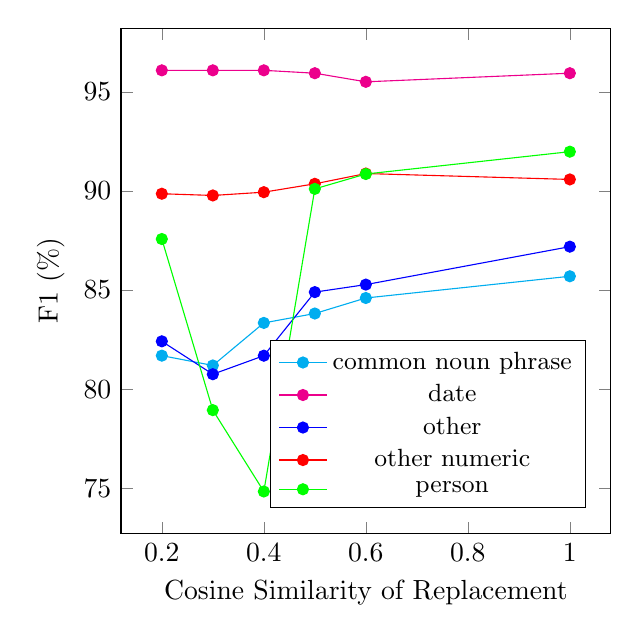
\begin{tikzpicture}
\begin{axis}[
	xlabel=Cosine Similarity of Replacement,
	ylabel=F1 (\%),
	width=7.8cm,height=8cm,
    legend style={at={(0.95,0.05)},anchor=south east,font=\small}
    ]

% Add values and attributes for the first plot
\addplot[color=cyan,mark=*] coordinates {
    (0.2, 81.689853992002)
    (0.3, 81.1945084254312)
	(0.4, 83.3417461660917)
	(0.5, 83.8159310839503)
	(0.6, 84.599337928678)
	(1.0, 85.6952249207913)
	
};

% Add values and attributes for the second plot
\addplot[color=magenta,mark=*] coordinates {
    (0.2, 96.0869565217391)
    (0.3, 96.0869565217391)
	(0.4, 96.0869565217391)
	(0.5, 95.9420289855072)
	(0.6, 95.5072463768116)
	(1.0, 95.9420289855072)
};

\addplot[color=blue,mark=*] coordinates {
    (0.2, 82.412886168088)
    (0.3, 80.7526601670349)
	(0.4, 81.6875630583188)
	(0.5, 84.8958705096486)
	(0.6, 85.2745770750729)
	(1.0, 87.1891342919242)
    
};

\addplot[color=red,mark=*] coordinates {
    (0.2, 89.8596228700561)
    (0.3, 89.7731594032172)
	(0.4, 89.9384801977591)
	(0.5, 90.3606485220866)
	(0.6, 90.8793150533339)
	(1.0, 90.5816337151901)

};

\addplot[color=green,mark=*] coordinates {
    (0.2, 87.5747707808863)
    (0.3, 78.9406378787976)
	(0.4, 74.8347323133535)
	(0.5, 90.1048032491703)
	(0.6, 90.855921375979)
	(1.0, 91.9824805135879)

};

\legend{common noun phrase, date, other, other numeric, person}
\end{axis}
\end{tikzpicture}
\caption{F1 for increasing levels of cosine similarity across five question categories.}
\end{figure}

In our experiments, looking at the relationship between cosine similarity and accuracy, we saw very similar results to what we hypothesized.

\subsection{Overall Results}

For cosine similarity levels 0.3 through 0.6 we saw an approximately linear decreasing relationship between the cosine similarity and the accuracy of the model. This decreasing trend shows that our model does utilize semantic meaning when predicting answers to the SQuAD1.1 question tasks. In our experiments, the prediction accuracy ranged from a low of approximately 75\% accuracy to a high of nearly 90\% accuracy. Because the accuracy did not dip below 75\%, we are led to believe that there is still a fairly strong reliance on syntactic structure, otherwise we would expect the drop to be much larger.

However, one outlier we noticed was at the 0.2 cosine similarity level. When modifying the question (with or without modifying the context) we saw a sharp increase in accuracy where before there had been a decrease. We saw the sharpest change when looking at modifications to the question only. The trend remained linearly downward for the context only category, and the question + context category had a less sharp increase. This leads us to believe that this increase is due to the change in the question. We are unsure why the question changes at a 0.2 cosine similarity level would cause this when none of the higher cosine similarities did.

\begin{figure}[h]
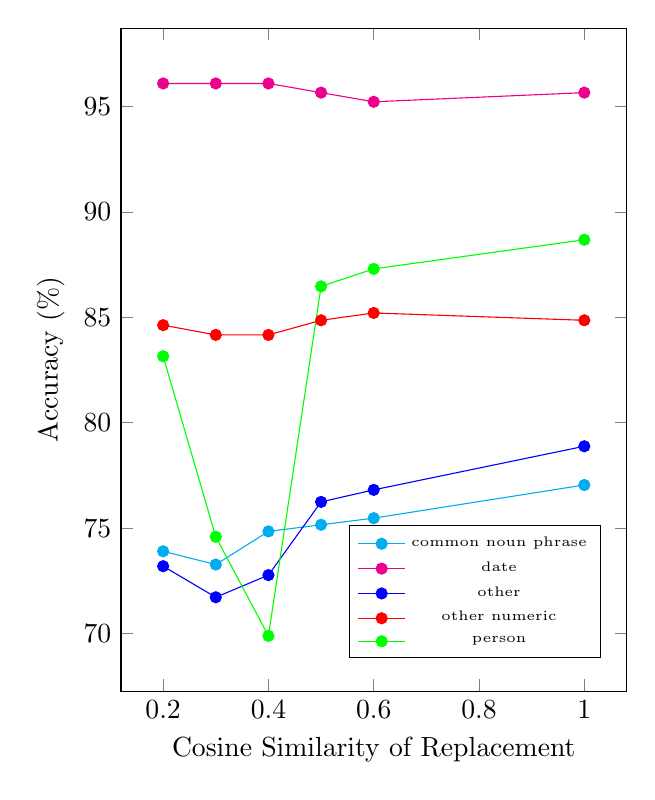
\begin{tikzpicture}
\begin{axis}[
	xlabel=Cosine Similarity of Replacement,
	ylabel=Accuracy (\%),
	width=8cm,height=10cm,
    legend style={at={(0.95,0.05)},anchor=south east, font=\tiny}
    ]

% Add values and attributes for the first plot
\addplot[color=cyan,mark=*] coordinates {
    (0.2, 73.8993710691824)
    (0.3, 73.2704402515723)
	(0.4, 74.8427672955975)
	(0.5, 75.1572327044025)
	(0.6, 75.4716981132076)
	(1.0, 77.0440251572327)
	
};

% Add values and attributes for the second plot
\addplot[color=magenta,mark=*] coordinates {
    (0.2, 96.0869565217391)
    (0.3, 96.0869565217391)
	(0.4, 96.0869565217391)
	(0.5, 95.6521739130435)
	(0.6, 95.2173913043478)
	(1.0, 95.6521739130435)
    
};

\addplot[color=blue,mark=*] coordinates {
    (0.2, 73.1924614505997)
    (0.3, 71.719017704169)
	(0.4, 72.7698458023986)
	(0.5, 76.2421473443746)
	(0.6, 76.8132495716733)
	(1.0, 78.8806396344946)

};

\addplot[color=red,mark=*] coordinates {
    (0.2, 84.6242774566474)
    (0.3, 84.1618497109827)
	(0.4, 84.1618497109827)
	(0.5, 84.8554913294798)
	(0.6, 85.2023121387283)
	(1.0, 84.8554913294798)

};

\addplot[color=green,mark=*] coordinates {
    (0.2, 83.1491712707182)
    (0.3, 74.585635359116)
	(0.4, 69.8895027624309)
	(0.5, 86.46408839779)
	(0.6, 87.292817679558)
	(1.0, 88.6740331491713)

};

\legend{common noun phrase, date, other, other numeric, person}
\end{axis}
\end{tikzpicture}
\caption{Accuracy for increasing levels of cosine similarity across five question categories.}
\end{figure}

\subsection{Question Category Analysis}

When looking at these trends in five of the ten categories discussed earlier (``common noun phrase,'' ``date,''  ``other,''  ``other numeric,''  and ``person''), we saw that some of these categories of questions were impacted much more severely by our substitutions, while others remained relatively constant. The ``other'' category is the largest of the categories and that line serves largely as a reference for the general trends in the dataset, as it contains all of the questions we could not categorize through data processing.

The categories we saw the least change in were ``date'' and ``other numeric'', which makes sense as for this sort of question we'd expect the model to lean more heavily on syntax. We believe that answers to those kinds of questions are fairly obvious from a context's syntax alone. The ``common noun phrase'' category seemed to largely mirror ``other'' (the general trends in the dataset), which makes sense due to the wide range of questions that have answers that are ``common noun phrases''. The category we saw the steepest change in was ``person.'' This is the most interesting result from our category analysis, as these questions were fairly clear cut (all containing some variation of ``who,'' ``who is,'' or ``whose''), and this result is very unexpected. It seems unperturbed at 0.6 and 0.5, and then falls by 15 percentage points at 0.4 cosine similarity, before beginning to climb back up as the cosine similarity drops further.

This category analysis shows that different types of questions are affected by perturbations in the semantic meaning in different ways. For example, date and numeric based questions are not affected at all, while questions about people are strongly affected.



\section{Discussion}
We drew two important conclusions from our experiments. First, while we saw a general trend in decreasing accuracy with decreasing cosine similarity, the model still performed close to baseline performance. This suggests that verb semantics is not essential to the model's prediction mechanism, as preservation of syntax is enough to keep the results within a 10\% range of baseline performance. 



Second, we found that question type had a significant effect on the model's performance on adversarial inputs. We saw a significant decrease in accuracy in answering perturbed ``person'' questions, and an overall increase in accuracy when answering perturbed ``date'' questions. Clearly, the relative importance of syntax and semantics to model performance on language understanding tasks depends on the nature of the task, and even the specific conformation of the inputs within one task.  



\section{Conclusion and Future Work}

Our analysis left us with some questions that we would be interested in exploring in future courses. The first major question relates to the upward spike we saw at 0.2 cosine similarity in Figures 1 and 2. We assume that this is due to the mid-range of cosine similarities being the most chaotic, while the lower cosine similarities start to look more like similar-but-opposite words like antonyms. However, we aren't able to confirm this without a more complete analysis of how our vector space behaves and what our cosine similarity selection is actually doing in terms of meaning.

The second major question is based on our category analysis. We saw very different behaviors dependent on the category of the questions. This begs the question of why some questions are more impacted than others. We proposed some possible explanations for this in our results section, but further work would be required to fully understand why these categories behave the way they do under the transformations we've applied. Specifically, we believe it would be useful to further divide the categories into smaller subcategories to narrow down which questions are and aren't impacted and examine the causes.

Our process for categorizing questions could also be improved upon and a larger group of questions could be categorized. We were only able to categorize less than 20\% of the dataset, and so the category analysis we were able to do was limited. More sophisticated and complete categorization could lend deeper insight into the behaviors we're seeing based on our perturbations.




% \begin{table}
% \centering
% \small
% \begin{tabular}{cc}
% \begin{tabular}{|l|l|}
% \hline
% \textbf{Cosine Similarity} & \textbf{Output}\\\hline
% \verb|{\"a}| & {\"a} \\
% \verb|{\^e}| & {\^e} \\
% \verb|{\`i}| & {\`i} \\ 
% \verb|{\.I}| & {\.I} \\ 
% \verb|{\o}| & {\o} \\
% \verb|{\'u}| & {\'u}  \\ 
% \verb|{\aa}| & {\aa}  \\\hline
% \end{tabular} &
% \begin{tabular}{|l|l|}
% \hline
% \textbf{Command} & \textbf{Output}\\\hline
% \verb|{\c c}| & {\c c} \\ 
% \verb|{\u g}| & {\u g} \\ 
% \verb|{\l}| & {\l} \\ 
% \verb|{\~n}| & {\~n} \\ 
% \verb|{\H o}| & {\H o} \\ 
% \verb|{\v r}| & {\v r} \\ 
% \verb|{\ss}| & {\ss} \\\hline
% \end{tabular}
% \end{tabular}
% \caption{Example commands for accented characters, to be used in, \emph{e.g.}, \BibTeX\ names.}\label{tab:accents}
% \end{table}



\bibliography{acl2019}
\bibliographystyle{acl_natbib}


\end{document}
